DaisyNFS is a verified, concurrent, and crash-safe file system, built on top of
GoTxn. This chapter describes its specification, implementation, and proof. A
key aspect of DaisyNFS is that the proofs of the file-system code use \emph{sequential
reasoning}, even though DaisyNFS is a concurrent file system. This is possible
due to a \emph{simulation-transfer theorem} that uses the strong
guarantee of GoTxn to enable verifying a system written with transactions using
a different proof strategy, so that the file-system proofs are carried out in
Dafny, a sequential verification-oriented programming language.

\section{Introduction}

File systems are important to implement correctly because applications rely on
them to safely store user data. Formal verification offers a promise of showing
that an implementation always meets its specification, including a crash safety
property that says the file system recovers correctly from a sudden crash and
reboot. However, efficient implementations are internally complicated,
especially because they support concurrency and aim to minimize disk writes.
This poses a challenge for formal verification: how can a proof cover
concurrency, crash safety, and functional behavior while remaining tractable for
a program the size of a file system?

Crash safety poses a challenge even without verification, so many file systems
use a technique called \emph{journaling} (sometimes called write-ahead logging)
to atomically write multiple objects to disk. An efficient journaling system
goes a long way towards correctness, but it does not protect the programmer from
all concurrency and crash safety reasoning. For example, consider allocating a
block using a combination of an in-memory allocator an on-disk state (to recover
the allocator state on reboot). Suppose one operation is freeing a block from a
file while a concurrent operation is allocating and using it. If the system
crashes, it is possible that the allocation and its writes succeed but the
freeing is aborted, resulting in the same block being part of two files.

The main contribution of this paper is a file-system design that \emph{isolates
crash safety and concurrency reasoning} to a transaction-system
implementation. We take inspiration from databases, which provide SQL
transactions to applications to avoid such tricky concurrency and crash
reasoning when using the database, except in this case the transactions help the
file-system implementation safely access the disk. Unlike existing designs, we
wrap all the file-system data structures and logic inside a transaction. The
benefit of this design is that it is especially verification friendly since it
supports \emph{sequential proofs} for the body of each transaction. Sequential
proofs keep the proof burden manageable even with an efficient implementation
which supports many features, such as large files and in-place updates of
serialized metadata.

There are two challenges in realizing this design. First, how can the entire
file system be implemented using transactions? Ordinarily file systems have some
shared mutable state that is independent of the journal --- the allocator is one
such piece of state that gives rise to the running bug example. We address this
issue by not relying on atomicity of the allocator and instead validating its
results with the journal (experiments demonstrate this has only a small
performance impact). Some operations, like freeing, can require a large number
of disk writes that might not fit in a transaction. We implement freeing using
multiple transactions; a first transaction logically deletes a file, and then
asynchronously the implementation can run transactions that recover space from
the file but have no other visible effect.

The second challenge is how to implement and prove the transaction system
itself. The performance and concurrency of the overall system can only be as
good as the transaction system, so efficiency and fine-grained locking are
important. To that end we start with GoJournal~\cite{chajed:gojournal}, a
verified journaling system that gets good performance and supports concurrent
access to objects smaller than the disk's block size (assumed to be 4KB).
GoJournal leaves concurrency control to the caller, which our transaction system
implements using a standard two-phase locking implementation.

There are two difficulties in proving the transaction system correct using the
GoJournal specificationh. First, this implementation cannot make all
transactions appear sequential; consider a simple example of a transaction that
increments a global variable unknown to the two-phase locking code. Instead, we
formalize a contract specifying rules for which transactions are legal and
assume the caller issues legal transactions in the correctness proof. Second,
most textbook proofs of two-phase locking work by showing that a global conflict
graph between transactions is cycle-free, which implies that the transactions
are serializable. Our proof needs to be tied to the implementation and in
particular the GoJournal specification based on separation logic, so we give a
new proof of two-phase locking's correctness using lock invariants and local
rather than global reasoning.

The verified artifact from this work is \sys, which implements a Network File
System (NFS) server on top of a bare disk and comes with a proof that clients
observe that each operation follows the NFS specification as laid out in RFC
1813. Operations appear atomic despite concurrency and crashes. Clients can use
the Linux or macOS NFS client to mount \sys like any other file system and
interact with it using the usual POSIX API.
As an end-to-end check that our formalization of NFS is
accurate and the implementation is reasonably complete, we tested with both Linux
and macOS clients running a variety of programs and under interactive usage.

A significant benefit of this file-system design is that it permits using the
sharpest tool for each part of the proof: while we use
Perennial~\cite{chajed:gojournal}, a program logic for crash safety and concurrency, for the
transaction system's proof, we use Dafny~\cite{leino:dafny}, a verification-aware
programming language with powerful automation, for the file-system operations.
Dafny is a purely sequential language, but we are able to use it despite this
limitation since the transaction system's proof guarantees transactions behave
sequentially. The value of
sequential proofs can be seen in the proof-to-code ratio for the transaction
system, which is $18\times$, versus the Dafny proofs which required about
$2\times$ as many lines of proof as code. Further evidence can be seen in the
incremental development of DaisyNFS, which we elaborate on in
\autoref{sec:eval:incremental}.

% \joe{Should some of this paragraph's ideas move up to the part where we first argue for the split and describe Dafny as the best tool for the other side?}
% The verification approach we propose makes the proof much simpler. The
% productivity from doing the proofs in Dafny enabled us to rapidly prototype and
% add features incrementally, including triply-indirect blocks, directories, and
% efficient in-memory data structures. These features were important to get good
% performance and support a range of applications. As some quantitative evidence
% for simpler proofs, \sys's \sys's proof is about $2\times$ as many lines as its
% implementation, a rough measure of proof complexity. For comparison, this is
% significantly lower than the overhead in our transaction system (about
% $18\times$) and comparable to the proof:code ratio for the three prior systems
% verified in Dafny, IronClad~\cite{hawblitzel:ironclad} with $4.8\times$,
% IronFleet~\cite{hawblitzel:ironfleet} with $3.6\times$, and VeriBetrKV~\cite{hance:veribetrkv} with
% $4\times$.\footnote{These numbers exclude refinement proofs in these systems
% written on top of the implementation specs, since \sys does not have any
% comparable proofs.}

To evaluate DaisyNFS's performance, we compare it to that of the Linux NFS server
exporting an ext4 file system. \sys achieves almost the same performance as
Linux with the ext4 \cc{data=journal} option (which gives the same crash-safety
guarantees as \sys), across a variety of benchmarks run on top of a fast NVMe
drive. The comparable performance is due to the efficiency of GoJournal and
adding little overhead in the file-system code (e.g., updating data structures
in place to avoid copying). We do note that ext4's default \cc{data=ordered}
mode can get about $2\times$ better throughput for data-heavy workloads, at the
cost of relaxed guarantees on crash.

The contributions of this paper are:
\begin{itemize}
  \item A file-system design that uses transactions in a principled way to
  isolate crash safety and concurrency to the transaction system and use
  sequential proofs for file-system logic.
  \item A contract formalizing which transactions the transaction system can
  make atomic, and a proof of its correctness under this contract.
  \item DaisyNFS, a verified file system and transaction system that implement
  these ideas. A performance evaluation shows that DaisyNFS gets performance
  comparable to Linux ext4 exported over NFS.
\end{itemize}

Our approach and DaisyNFS have some limitations. We do not support NFS unstable
writes, which improve performance by not committing writes to stable storage
until explicitly requested. The proof approach relies on showing that
transactions appear to execute sequentially; this prevents us from modifying state
outside the transaction system (and reasoning about the interaction) where that
would get better performance. The transaction system does not have a proof of
liveness, and we do not prove that transactions avoid deadlock. Our NFS
implementation does not cover the entire API, such as symbolic and hard links,
the ``weak-cache consistency'' metadata to support client-side caching, or
paginated \cc{READDIR}; we believe all of these could be implemented and
specified with the same approach, but have not done so in our prototype.

\section{System design}%
\label{sec:daisy:system}

\begin{figure}
  \center
  \begin{tikzpicture}[>=latex, node distance=1.25cm]

 \tikzset{
    genericnode/.style={rectangle,draw,minimum width=2cm, minimum height=.85cm, align=center,},
    layer/.style={
      genericnode,
      alias=genericnode,% <- alias added
      label={[anchor=south west,shift={(genericnode.north west)},inner sep=2pt]{\tiny #1}}% position the label using the alias
    }}

%\tikzstyle{layer}=[rectangle, draw, minimum width=2cm, minimum height=.85cm, align=center];
\tikzstyle{genlayer}=[dashed, layer={}];
\tikzstyle{edge}=[->,thick];

\draw node (dispatch) [layer=Go] {Dispatch Loop};
\draw node (goout) [genlayer,below of=dispatch] {Go output};
\draw node (txn) [layer=Go,below of=goout] {GoTxn};

\draw node (coq) [left=1.5cm of txn, align=center] {Verification \\ in Perennial};
\draw node (dafny) [left=1.25cm of goout, layer=Dafny] {File-system \\ Operations};

\draw node (out) [below=1cm of txn] {\texttt{daisy-nfsd} binary};

\draw [thick] (dispatch.south) -- (goout.north);
\draw [thick] (goout.south) -- (txn.north);
\draw [edge] (txn.south) -- node[right] {\texttt{go build}} (out.north);
\draw [edge] (txn.west) -- (coq.east);

\draw [edge] (dafny.east) -- node[above] {\texttt{dafny}} (goout.west);


\end{tikzpicture}

  \caption{The structure of DaisyNFS.}
  \label{fig:system}
\end{figure}

As shown in \cref{fig:system}, DaisyNFS is implemented in three layers:
1) a dispatch loop that speaks the NFS wire protocol and calls the
appropriate method for each operation; 2) a Dafny class that
implements each method; and 3) a transaction system that applies the
updates of each method to the disk atomically.  The dispatch loop is
unverified; we assume that the server correctly decodes messages,
calls the right method for an operation, and encodes the response. The
middle layer implementing the file-system operations is written
and verified in Dafny, which has a backend for Go.  The
third layer is directly written in Go and verified using Coq and
Perennial.  By implementing the file system on top of the transaction
system, we can implement each NFS method in Dafny as sequential code
calling into a concurrent transaction system library. The NFS
operations supported by DaisyNFS are listed in \cref{fig:nfs}.

%% We focus on the
%% design of the transaction system here, but the file system also has several
%% internal abstractions. These abstractions are primarily interesting in a
%% verification context so we discuss them later in \cref{sec:daisy:design}.

%% The file-system implementation calls the transaction system to store all
%% file-system data, ensuring that it is written atomically and durably.
%%
\begin{figure}
  \centering
  \begin{tikzpicture}[>=latex]

  \tikzstyle{circlog}=[thick,rectangle, draw,minimum height=1cm, align=center];

  \node[circlog,minimum width=1cm,
       label={[label position=below, align=center]Super\\block}] (logger) {};
  \node[circlog,minimum width=1.7cm, right=0cm of logger,
    inner sep=0pt,
    rectangle split,
    rectangle split every empty part={},
    rectangle split parts=6,
    rectangle split empty part width={.2cm},
    rectangle split horizontal,
       label={[label position=below, align=center]20 inode\\ blocks}] (installer) {};

  \node[circlog, right=0cm of installer,
    inner sep=0pt,
    rectangle split,
    rectangle split every empty part={},
    rectangle split parts=20,
    rectangle split empty part width={.1cm},
    rectangle split horizontal,
       label={[label position=below, align=center]30 allocator\\ bitmap blocks}] (log) {};


  \node[circlog,minimum width=3.2cm, right=0cm of log,
    inner sep=0pt,
    rectangle split,
    rectangle split every empty part={},
    rectangle split parts=3,
    rectangle split empty part width={1.15cm},
    rectangle split horizontal,
       label={[label position=below, align=center]data blocks\\ (remainder of disk)}] (log2) {};

  \draw [line width=.05cm,black,transform canvas={yshift=.25cm}] (installer.south west)+(0,-.5cm) -- (installer.north west);
  \draw [line width=.05cm,black,transform canvas={yshift=.25cm}] (log.south west)+(0,-.5cm) -- (log.north west);
  \draw [line width=.05cm,black,transform canvas={yshift=.25cm}] (log2.south west)+(0,-.5cm) -- (log2.north west);

%  \tikzstyle{circlog}=[thick,rectangle, draw,minimum height=1.5cm, align=center];
%
%  \node[circlog,minimum width=1.2cm,
%       label={[label position=below, align=center]Super\\block}] (logger) {};
%  \node[circlog,minimum width=1.7cm, right=0cm of logger,
%       label={[label position=below, align=center]20 inode\\ blocks}] (installer) {};
%
%  \node[circlog,minimum width=2.0cm, right=0cm of installer,
%       label={[label position=below, align=center]30 allocator\\ bitmap blocks}] (log) {};
%
%  \node[circlog,minimum width=3.4cm, right=0cm of log,
%       label={[label position=below, align=center]data blocks\\ (remainder of disk)}] (log) {};

%  \node[] at (-0.45cm,-1cm) {$\uparrow$ 0};
%  \node[] at (4.2cm,-1cm) {$\uparrow$ 513};

%  \draw [decorate,decoration={brace,mirror,amplitude=10pt},xshift=-4pt,yshift=0pt]
%    (-0.45cm,-1.2cm) -- (4cm,-1.2cm) node [black,midway,yshift=-0.6cm]
%    {\scc{circular}};

\end{tikzpicture}

  \caption[File-system disk layout]%
  {The layout of the file system on top of the transaction system's
    disk. The number of inode blocks and data bitmap blocks are compile-time
    constants, but easy to change without affecting the proofs.}
  \label{fig:layout}
\end{figure}

The file system is responsible for implementing files and directories
onto an array of disk blocks that is exported by the transaction
system.  The disk layout used by the file system is shown in
\cref{fig:layout}, with regions for inode blocks, bitmap blocks,
and data blocks for files and directories. This figure is in terms of
the disk exported by the transaction system; the transaction system
itself reserves a prefix of 513 blocks for the write-ahead log.

The high-level organization of the file system separates three concerns, each
building upon the previous: (1) implementing indirect blocks to support large
files; (2) implementing byte-granularity
reads and writes on top the block-granularity interface below; and (3) implementing
directories by encoding them as files with a special type together with
operations to manipulate those files. \Cref{sec:daisy:design} explains the
internals of the file-system design in more detail, alongside the structure of
the Dafny proof.

%% Each
%% operation takes place in a single transaction at run time, but this transaction
%% is built up by calling methods through several abstraction layers before
%% eventually producing a sequence of transactional reads and writes.

Recall that GoTxn supports accessing objects smaller than a block. DaisyNFS uses
three sizes of objects: bit objects comprise the inode and block allocators,
128-byte objects are used to represent inodes, and full 4KB blocks are used for
file and directory data (including indirect blocks). The file system statically
allocates regions for these three kinds of blocks, much like ext4.

Acquiring multiple locks during a transaction creates the possibility
for deadlocks, for example if two threads acquire a pair of locks in the opposite
order. The two-phase locking implementation does not implement a
specific lock acquisition order, leaving it to the file system to
avoid deadlock --- the most interesting case is \cc{RENAME}, which is discussed
in more detail in \cref{sec:dafny:rename}.

\section{Specifying DaisyNFS}%
\label{sec:daisy:spec}

The specification for DaisyNFS is a state machine describing an ideal NFS server in
the form of an abstract state and a transition for each operation. The
implementation of DaisyNFS is a binary \cc{daisy-nfsd} that implements the NFS
protocol, running on top of a
disk. Then the DaisyNFS correctness
theorem is a \emph{refinement} property, which intuitively says that
for any interaction with the
implementation, the ideal, atomic NFS state machine could produce the responses;
this section shortly gives a more formal definition.
As a result a client interacting with the server can pretend
that it is the NFS state machine and ignore the complexities of its
implementation.

\subsection{Formalizing NFS}%
\label{sec:daisy:nfs}

RFC 1813 specifies the NFS protocol, which we make mathematically precise with a
state-machine representation defined in Dafny.
The formalization requires first
defining an abstract state, and then a transition for each
NFS operation that specifies how it changes that state and what return
values are allowed. While most of the specification is deterministic,
some operations have to be specified with non-determinism; for
example, we allow returning an out-of-space error in many operations,
and the specification allows any timestamp to be picked for the
current time. The RFC is precise about arguments and allowed return
values, and the text is good about explaining the intended behavior,
but it does not separately describe an abstract state to make that behavior
mathematically precise.  We define
the NFS server state as shown in \cref{fig:dafny-state}.

\begin{figure}[ht!]
\begin{verbatim}
// the abstract state of the file system
type FilesysData = map<Ino, File>

datatype File =
  | ByteFile(data: seq<byte>, attrs: Attrs)
  | Dir(dir: map<FileName, Ino>, attrs: Attrs)

type Ino = uint64
type FileName = seq<byte>
datatype Attrs = Attrs(mode: uint32, ...)
\end{verbatim}
\caption{Dafny definition of the NFS server state (simplified).}
\label{fig:dafny-state}
\end{figure}

This definition says that an NFS server conceptually maintains a mapping from
inode numbers to files, where a file can either be a regular file with
bytes, or a directory. Both types of files have a number of attributes, storing
metadata like the file's mode (permission bits) and modification time. A
directory is a partial map from file names
(which are just bytes) to inode numbers. Note that DaisyNFS doesn't
represent the file system as a tree but as a collection of
links, which is sufficient to model all NFS operations, because
NFS clients resolve path names.

% \mfk{the rest of this
%   paragraph is lacking a clear narrative.}
% In any case a
% tree wouldn't be a sufficient state for NFS since modifying one file
% affects any other hard links to the same file (note though that DaisyNFS
% does not currently support hard links).

The NFS state machine models each operation as a non-deterministic transition
that answers when it is allowed for an operation to change the state from
\cc{fs} to \cc{fs'} and return \cc{r}. The return value is always wrapped in a
\cc{Result} type, which can be either \cc{Ok(v)} for a normal return or an error
code for one of the errors defined in the standard. The file system systematically guarantees
that the state is unchanged when an operation returns an error (though this is
stronger than what the RFC mandates); the transaction system makes this easy to
achieve by aborting the whole transaction. For example,
\cref{fig:getsz} shows the
specification for a (hypothetical) \cc{GETSZ} operation that returns the size of
the inode \cc{ino}.

\begin{figure}[ht]
\begin{verbatim}
predicate GETSZ_spec(ino: Ino, fs: FilesysData,
  fs': FilesysData, r: Result<uint64>)
{
  fs' == fs &&
  (r.ErrBadHandle? ==> ino !in fs) &&
  (r.ErrIsDir? ==> (ino in fs) && fs[ino].Dir?) &&
  (r.Ok? ==> (ino in fs) && fs[ino].ByteFile? &&
             r.v == |fs[ino].data|)
}
\end{verbatim}
  \caption[Transition-system specification for a hypothetical \cc{GETSZ} operation.]%
  {Specification of a hypothetical \cc{GETSZ} operation, a simplification
  of the real \cc{GETATTR} operation. When \texttt{GETSZ\_spec(ino, fs, fs', r)}
  returns true, it is valid when the server receives \cc{GETSZ(ino)} to transition from
the state \cc{fs} to \cc{fs'} and return \cc{r}. The return value can be an
error (e.g., \cc{r.ErrBadHandle?}), or if \cc{r.Ok?} holds then \cc{r.v} is the
\cc{uint64} return value from the operation.}
\label{fig:getsz}
\end{figure}

There are four clauses in the specification. The first just says that this
operation is read-only. The second is one possible error: if the server returns
\cc{ErrBadHandle}, then \cc{ino} is not allocated. The third is a different
error, which says this operation returns \cc{ErrIsDir} if passed a directory inode.
Finally the fourth clause says that if the operation is successful, it returns the
length of the data in \cc{fs[ino]}. Dafny checks several consistency properties
of this specification itself; for example, a use of \cc{fs[ino]} only compiles
if the specification earlier implies \cc{ino in fs}.

We developed a state-machine model of the regular file and directory operations
in NFS in this style, including specifying what certain errors
signify. \Cref{fig:nfs} lists the entire NFS API and what parts are verified in
DaisyNFS.
The file system has unverified implementations \cc{FSINFO} and \cc{PATHCONF}, which give the client static
configuration information about the file system (for example, the maximum supported
write size or the maximum path length). These return constants and thus have no
associated proof. DaisyNFS also implements \cc{FSSTAT} to report total and free space,
but it does not have a meaningful specification.


\renewcommand{\check}{\textcolor{ForestGreen}{\checkmark}}
\newcommand{\nope}{\textcolor{Maroon}{\ding{55}}}

\begin{figure}
\small \centering
\begin{tabular}{@{~}ll@{}c@{~}}
  \toprule
  \bf Category & \bf Operations & \bf Verified \\
  \midrule
  \textit{File and directory ops}
  & \cc{GETATTR}, \cc{SETATTR}, \cc{READ}, \cc{WRITE} & \check \\
  & \cc{CREATE}, \cc{REMOVE}, \cc{MKDIR}, \cc{RENAME} & \check \\
  & \cc{LOOKUP}, \cc{READDIR} & \check \\

  \textit{Unsupported features}
  & \cc{READLINK}, \cc{SYMLINK}, \cc{LINK}, \cc{MKNOD} & \nope \\
  & \cc{READDIRPLUS}, \cc{ACCESS} & \nope \\

  \textit{Configuration}
  & \cc{FSINFO}, \cc{PATHCONF}, \cc{FSSTAT} & \nope \\

  \textit{Trivial operations}
  & \cc{NULL}, \cc{COMMIT} & \check \\

  \bottomrule
\end{tabular}
\caption{NFS API and which operations DaisyNFS supports and verifies.}
\label{fig:nfs}
\end{figure}

DaisyNFS could support some of the remaining operations with some more effort.
A symbolic link is essentially a file that holds a path, which is created with
\cc{SYMLINK} and can be read with
\cc{READLINK}. \cc{MKNOD} similarly creates a new type of special file that
consists of a major and minor device number.
Specifying these operations would require mostly mechanical changes to the
specification to accommodate the new file types.
\cc{LINK} is more complicated because in addition to tracking
the link count of every file in the state, the specification for \cc{REMOVE}
needs to say that the link count is decremented and that the file is deleted if
its link count drops to zero.

The current implementation of \cc{READDIR} always returns the entire directory,
which is impractical for large directories; NFS supports a paginated API, where
\cc{READDIR} returns some directory entries and then an offset to resume
iteration. The complication with this API is that the directory could change
between reads, so the interface has provisions to handle
this kind of \emph{iterator invalidation} and the specification would need
similar adaptations. We believe it would be possible to adapt the work in
SibylFS~\cite{ridge:sibylfs}, a specification for the POSIX file-system API, which gives a
specification for the analogous \cc{readdir} system call. DaisyNFS does not
support \cc{READDIRPLUS}, which differs from \cc{READDIR} only in that it also
returns attributes along with names and inode numbers.

\subsection{Specifying correctness for DaisyNFS}%
\label{sec:daisy:refinement-spec}

\begin{figure}[ht]
\small
\centering
\begin{tabular}{@{~}llr@{~}}
\toprule
\bf Layer & \bf Operations & \\
\midrule
  NFS
      & \cc{CREATE(d_ino, name)}, \cc{READDIR(d_ino)}, \dots & \cref{sec:daisy:spec} \\
  Txn
      & \cc{Read(tx, a, sz)}, \cc{Commit(tx)}, \cc{Alloc(a)},
        \dots & \cref{sec:txn:api} \\
  Disk
      & \cc{Read(a)}, \cc{Write(a, b)} & \\
\bottomrule
\end{tabular}
\caption{API layers of DaisyNFS.}
\label{fig:layers}
\end{figure}

The previous section (\cref{sec:daisy:nfs}) defines the transition system for NFS,
which this section relates to the actual DaisyNFS implementation in order to
define correctness. The definition uses the ideas from
\cref{sec:txn:refinement-def,sec:txn:go-layers}, namely the definition of
refinement and the definition of $\gooselayer{X}$, where X is instantiated
separately with both the Txn and NFS layers. \gooselayer{NFS} has a primitive for each operation supported by
DaisyNFS, and the semantics of these primitives is defined to be the NFS
transition system written in Dafny. Implicit in such a semantics is that each
operation is atomic both with respect to other threads and on crash.

With the NFS layer we can model a \emph{server loop} that recovers the
file-system state, then repeatedly accepts a new request, processes it with the
appropriate NFS transition, and sends the reply back. Let us denote this server
loop with $\snfs : \gooselayer{NFS}$. Note that when this (abstract) server
processes an NFS operation, it does so by definition atomically, and its state
is again by definition preserved on crash. $\snfs$ can be viewed as an
abstraction of the following pseudo-code that represents the essence of the
real \cc{daisy-nfsd} binary:

\begin{minted}[linenos]{go}
// this is the core of daisy-nfsd
func main() {
  tx := txn.Recover()
  fs := filesys.Recover(tx)
  for {
    req := GetRequest()
    go func() {
      switch req.Op {
      case CREATE:
        ret := fs.CREATE(req.Args)
        SendReply(req, ret)
      case LOOKUP:
        ret := fs.LOOKUP(req.Args)
        SendReply(req, ret)
      // ... other cases ...
      }
    }()
  }
}
\end{minted}

This code starts by recovering the state of the system, starting with the
transaction system on line 3 and then continuing on to the file-system state on
line 4. Then it repeatedly accepts new requests from the network, abstracted
with \cc{GetRequest()} (including parsing the NFS wire protocol). These requests
are each processed in a background thread due to the goroutine spawned on line
7. The processing for each request dispatches to the appropriate file-system
operation (e.g., lines 10 and 13). The implementations of these operations are
compiled from Dafny to Go and then linked with the transaction system.

The term $\snfs$ represents the abstract version of this loop where, for example,
the entire call to \cc{fs.CREATE} is an atomic primitive. In the Dafny code,
this corresponds to an entire method that calls the GoTxn API. We can think of
each method as having a corresponding GooseLang term that represents its
implementation at the Txn layer of abstraction, for example
$\mathit{CREATE} : \gooselayer{Txn}$ might model the \cc{fs.CREATE} method.
These constructions are all for the sake of the proof argument; it is part of
the assumptions of the proof that every method can be modeled using GooseLang.
Next, let $\sdfy$ denote the same overall server dispatch loop with
methods at the GoTxn abstraction level. Finally, the lowest-level model of the
server is derived by combining the Dafny implementation with the actual GoTxn
implementation, which we write as $\linkedcode$.

$\linkedcode$ and $\snfs$ are both models of the \cc{daisy-nfsd} server binary's
behavior. The former is a model of its implementation running on top of a disk,
while the latter is its specification at the level of NFS methods. These two
together are enough to state the overall DaisyNFS correctness theorem:
%
\begin{theorem}[DaisyNFS correctness] $\linkedcode \refines \snfs$; that is, the
  DaisyNFS code follows the NFS specification.
  Initialization requires initializing the
  transaction system on an empty disk and then running the \cc{Init}
  constructor for the file-system. Subsequently the system boots by recovering the
  transaction system and then the file system with its \cc{Recover} constructor.
  \label{thm:daisy}
\end{theorem}

This theorem connects the server's implementation at the disk layer,
$\linkedcode$, which combines a model of the Dafny code with the GoTxn
implementations, to the most abstract version of the server $\snfs$ which by
definition atomically processes operations, preserves data on crash, and follows
the NFS state machine written in Dafny. \Cref{sec:daisy:proof} explains how this
specification is proven. The basic idea is that the Dafny reasoning relates
$\sdfy$ to $\snfs$ with a sequential proof, and GoTxn guarantees that sequential
reasoning for transactions is sufficient to guarantee the whole system satisfies
concurrent, crash-safe refinement due to the atomicity of every transactions.

\section{Verifying DaisyNFS using Dafny}
\label{sec:daisy:proof}

A key contribution of DaisyNFS is a proof structure that isolates concurrency and crash
reasoning to the transaction system. The proof works in two steps. First, a
\emph{simulation transfer} theorem extends GoTxn's transaction refinement to show
how transactions enable sequential reasoning for an arbitrary system implemented on
top (\cref{sec:daisy:simulation-transfer}). Second, simulation transfer is
applied to DaisyNFS and its sequential reasoning carried out in Dafny
(\cref{sec:daisy:proof-dafny}).

\subsection{Simulation transfer}%
\label{sec:daisy:simulation-transfer}

The GoTxn specification from \cref{sec:txn:spec} uses transaction refinement to
capture that transactions are atomic in the sense that every interleaved
execution has a corresponding execution where each transaction runs all at once.
This section describes a \emph{simulation transfer} theorem, proven in Coq, that
uses transaction refinement to show how GoTxn enables \emph{sequential
reasoning} for a system implemented with transactions on top.

The idea behind the simulation transfer specification is to express that a system
verified using sequential reasoning for each transaction is also correct when
run concurrently through GoTxn --- intuitively, this follows from the atomicity
provided by transaction refinement.
% , at which point the sequential reasoning
% applies, but we have a more precise and formal proof in Coq.
To make this precise, we define formally what we mean by
``sequential reasoning''. Suppose we have an
implementation of layer $S$ using operations from $T$. The implementation $i$
consists of a function $i(\opv) : \gooselayer{T}$ for each operation $op \in S$. The statement
$\seqrefinement \targ{T, S}(i)$ says that $i$ is a correct sequential
implementation of $S$ using $T$. The effect of each operation is given by a
transition relation $\sigma \overset{\opv}{\leadsto} \sigma'$ that is part of the layer
$S$. To specify correctness under crashes, the
definition of sequential refinement refers to $\crash(\sigma, \sigma')$, which is a
layer-specific crash transition that models, for example, clearing the
contents of memory.

\begin{definition}
  The implementation $i : S \to \gooselayer{T}$ is a \emph{sequential
    refinement}, written
  $\seqrefinement \targ{T, S}(i)$, if there exists an abstraction relation
  $R : \Sigma_{S} \to \Sigma_{T} \to \textdom{bool}$ such that: \newline
(1) for every operation
  $op \in S$, the following sequential Hoare triple holds:
  \[
    \hoare{R(\sigma)}{i(\opv)}{\exists \sigma'.\, R(\sigma') \land \sigma \overset{\opv}{\leadsto} \sigma'},
  \]
(2) $\mathrm{init}(\sigma_{S}, \sigma_{T})$ implies
$R(\sigma_{S}, \sigma_{T})$, and \\
(3) if $R(\sigma_{S}, \sigma_{T})$ holds and $\crash(\sigma_{T}$, $\sigma_{T}')$,
then there exists a $\sigma_{S}'$ such that $R(\sigma_{S}', \sigma_{T}')$ and
$\crash(\sigma_{S}, \sigma_{S}')$.%
  \label{def:seqrefinement}
\end{definition}
%
Conditions (1) and (2) in this definition are standard for sequential
verification of refinement, while condition (3) is a standard condition for sequential crash-safety~\citep{chajed:argosy}. Though condition (3) requires the
abstraction relation to be preserved by crashes, the proof engineer does \emph{not} have to reason about crashes in the middle of operations.
% is a standard condition for sequential crash-safety~\cite{chajed:argosy}
% for sequential crash safety~\cite{chajed:argosy}.
The
diagram in \cref{fig:refinement:seq} depicts the main
refinement condition (1) diagrammatically.
% For example, it is fairly easy to use them to show
% that for any sequential program $p : \gooselayer{S}$, the traces of the code
% $\mathrm{link}(p, i)$ are a subset of the traces of the spec $p$ (we will not
% use exactly this theorem since we are interested in concurrent code using
% transactions).
% \tej{I mentioned this but maybe we don't want/need to say it?}. Such reasoning would be familiar in previous sequential verified
% systems like FSCQ~\cite{chen:fscq}, IronFleet~\cite{hawblitzel:ironfleet}, and
% VeriBetrKV~\cite{hance:veribetrkv}.

The simulation transfer theorem takes a proof of \emph{sequential} refinement
conditions for a system implemented using transactions and derives a
\emph{concurrent and crash-safe} refinement. Like transaction refinement, it is
stated as a theorem about an arbitrary program $p : \gooselayervar{Sys}$ using
the specification-level API.\@ To model that program using the transactions given
by implementation $i$, we write $\mathrm{link}(p, \atomiccomp i)$. The function
$(\atomiccomp i)(\opv) = \atomically{i(\opv)}$ wraps the implementation
$i(\opv)$ in an \cc{atomically} block. Physically this \cc{atomically} block
corresponds to running code in a pattern like the following, written using Go's
support for generics:
%
\begin{minted}{go}
type txnBody[T any] func(tx *Txn) (T, bool)
func runTxn[T any](f txnBody[T]) (v T, ok bool) {
  tx := Begin()
  v, ok := f(tx)
  if ok { tx.Commit() } else { tx.Abort() }
  return v, ok
}
\end{minted}

In order for simulation transfer to work, every transaction must satisfy some
conditions to ensure atomicity. We write $\safe(i(\opv))$ to say that $i(\opv)$ is a
valid transaction. The main restriction is that $i(\opv)$ cannot access global state
such as the heap, since the transaction system does not make such accesses
atomic; further details are discussed in \cref{sec:txn:transaction-refinement}.

\begin{theorem}[Simulation transfer]
  Let $\textdom{Sys}$ be a layer implemented using transactions with
$i : \textdom{Sys} \to \gooselayer{Txn}$, such that
$\seqrefinement\targ{\gooselayer{Txn}, \textdom{Sys}}(i)$ and
$\forall \opv.\, \safe(i(\opv))$ hold. Then
\[
  \forall p : \gooselayervar{Sys}, \linked{\mathrm{link}(p, \atomiccomp i)} \refines p.
\]
\label{thm:gotxn-transfer}
\end{theorem}
\nopagebreak

The theorem is about a program $p$ using some API $\Sys$, such as the server
loop for DaisyNFS seen in \cref{sec:daisy:refinement-spec}, and an
implementation $i$ of this API.\@
The conclusion is a refinement that uses $p$ as the \emph{specification}; recall
that the semantics of $p$ defines all the $\Sys$ operations to be atomic at this
layer. The left-hand side is the executable code for this program, derived in
two steps: first $\mathrm{link}(p, \atomiccomp i)$ takes each abstract operation
$\opv$ in $p$ and replaces it with $\atomically{i(\opv)}$, and second
$\linked{\mathrm{link}(p, \atomiccomp i)}$ takes the result of this process and
further replaces $\atomically{i(\opv)}$ with executable code that uses the GoTxn
implementation for each call to the Txn API and the \cc{runTxn} pattern above to
make the snippet atomic. The overall refinement says that this executable code
has a subset of behaviors of $p$, so that each operation is not only atomic but
follows the abstract specification of the $\Sys$ layer.

Simulation transfer is stated and proven in Coq. The proof builds on top of
transaction refinement. For every execution of the code, transaction refinement promises
a corresponding atomic execution of $\mathrm{link}(p, \atomiccomp i)$, and the
sequential refinement assumption is enough to show that the transactions
correctly simulate $p$ at the $\mathit{Sys}$ abstraction level.

\subsection{Using simulation transfer with Dafny}%
\label{sec:daisy:proof-dafny}

\newlength{\stepw}
\newlength{\dstepw}
\newlength{\nfstop}

Simulation transfer reduces verifying DaisyNFS's correctness to reasoning about
the transaction that implements each NFS operation. Because this reasoning is
sequential, we carry it out in Dafny, a verification-oriented programming language.
Let $\infs : \mathrm{NFS} \to \gooselayer{Txn}$ denote a model of the
Dafny implementation of each NFS operation, as a program using the GoTxn
interface. Note that this is merely a hypothetical model of the Dafny code,
since Goose does not support enough of Go to explicitly construct these terms in
GooseLang. The Dafny annotations on these methods prove sequential refinement
conditions that we will denote $\seqrefinementdfy(i)$, as
illustrated in \cref{fig:refinement}. This sequential refinement is indexed by
``dfy'' to indicate that it captures what is proven in Dafny. It is intended
that this obligation captures $\seqrefinement(i)$ from the simulation-transfer
theorem, but using a formal distinction always to say that the connection
between these definitions is trusted. Dafny checks the following lemma that
$\infs$ is correct, which will eventually be used to show the overall DaisyNFS
correctness theorem:
%
\nopagebreak
\begin{lemma} $\seqrefinementdfy(\infs)$ holds, as checked by Dafny.
  \label{thm:dafny}
\end{lemma}

We now state more formally what $\seqrefinementdfy$ means.
The Dafny code is implemented as a class with ghost variables for its abstract
state and an invariant that expresses the proof's refinement relation $R$
between the abstract state and its concrete state (which is limited to constants
and the transaction system's logical disk). The top-level interface is outlined
in \cref{fig:dafny-outline}. Condition (1) in the definition of
sequential refinement is encoded exactly in Dafny, using \cc{requires} and \cc{ensures}
clauses. Condition (2) for initialization and condition (3) for crashes relate
to the Dafny code in a slightly more subtle way.

\begin{figure}
  \begin{verbatim}
class Filesys {
  // the external abstract state
  ghost data: FilesysData;
  var txs: TxnSystem;

  // abstraction relation that relates txs.disk to data
  predicate Valid() { ... }

  // see text for these signatures
  constructor Init() { ... }
  constructor Recover() { ... }

  method GETATTR(ino: uint64) returns (r: Result<Attrs>)
    requires Valid() ensures Valid()
    ensures GETATTR_spec(old(fs), fs, ino, r) { ... }

  // ... methods for other NFS operations ...
}
  \end{verbatim}
  \caption{Outline of how the Dafny proof is expressed.}
  \label{fig:dafny-outline}
\end{figure}

\newcommand{\Op}{\mathcal{O}}

To describe how Dafny encodes this form of refinement, we start by describing its
specification transition system in more formal detail. The specification
transition system is
a triple $S = (\Sigma, \Op, \delta)$ where $\sigma \in \Sigma$ is a set of states,
$o \in \Op$ is a set of operations, and $\delta$ is a relation, where
$\delta(\sigma, o, \sigma', v)$ is true when in state $\sigma$ operation $o$ can
transition to $\sigma'$ and return $v$. To simplify the notation, the transition
system has a special operation $\mathsf{crash}$ to represent a crash transition.

\newcommand{\altsys}[1]{\tilde{#1}}

To define $S$, we build on a subset of its transitions $\altsys{S}$ that only
defines the methods of the Dafny class.
A state $\sigma \in \altsys{\Sigma}$ of this sub-transition system
consists of the values for all the ghost variables that define the API; in the
case of the file system this is just the \cc{data} field of type
\cc{FilesysData}, which was defined in \cref{fig:dafny-state}. Each NFS method and its
arguments is an operation $o \in \altsys{\Op}$, and predicates like \cc{GETSZ_spec}
define the transition relation $\altsys{\delta}$. Building on $\altsys{S}$, we
can now define $S$ by incorporating
initialization and recovery, which are implemented
in Dafny as \emph{constructors} \cc{Init} and \cc{Recover}. Constructors are
needed to set up the system's global constants, and to initially establish the
abstraction relation. Below we define $S$ in terms of $\altsys{S}$.
To define $\delta$, we write $\sigma \xrightarrow[v]{o} \sigma'$ to mean that
$\delta(\sigma, o, \sigma', v)$ is true, and let $\delta$ implicitly be false
elsewhere for undefined transitions.

\begin{figure}[ht!]
  \begin{mathpar}
  \begin{array}{llcl}
    &\Sigma &\defeq & \mathsf{UnInit} \ALT \mathsf{Running}(\sigma:
                      \altsys{\Sigma}) \ALT \mathsf{Crashed}(\sigma:
                      \altsys{\Sigma}) \\
    &\Op &\defeq & \mathsf{Init} \ALT \mathsf{Recover} \ALT \mathsf{Method}(o:
                   \altsys{\Op}) \\
    &\delta& \defeq& \mathsf{Running}(\sigma) \xrightarrow[v]{\mathsf{Method}(o)}
        \mathsf{Running}(\sigma') \text{ when } \sigma \xrightarrow[v]{o}

        \sigma' \text{ (in  $\altsys{\delta}$)} \\
    &&& \mathsf{UnInit} \xrightarrow{\mathsf{Init}} \mathsf{Running}(\sigma_0) \\
    &&& \mathsf{Crashed}(\sigma) \xrightarrow{\mathsf{Recover}} \mathsf{Running}(\sigma) \\
    &&& \mathsf{Running}(\sigma) \xrightarrow{\mathsf{crash}}
        \mathsf{Crashed}(\sigma') \text{ when } \sigma
        \xrightarrow{\mathsf{crash}} \sigma' \text{ (in  $\altsys{\delta}$)} \\
    &&& \mathsf{UnInit} \xrightarrow{\mathsf{crash}} \mathsf{UnInit} \\
    &&& \mathsf{Crashed}(\sigma) \xrightarrow{\mathsf{crash}} \mathsf{Crashed}(\sigma) \\
  \end{array}
  \end{mathpar}
  \caption[Formal definition of the Dafny specification transition
  system.]{Defining the specification transition system $S$ for the Dafny code,
    in terms of $\altsys{S}$ which only defines the transitions for the
    methods.}
  \label{fig:daisy:formal-spec}
\end{figure}

The transition system $S$ embeds $\altsys{S}$ in the transitions over
$\mathsf{Running}(\sigma)$, and these are the usual transitions during normal
operation. However, the Dafny code has to transition into the
$\mathsf{Running}(\sigma)$ state in two places: first the $\mathsf{Init}$
operation starts the system in state $\sigma_{0}$, and following a crash, the
system generally transitions from $\mathsf{Running}(\sigma)$ to
$\mathsf{Crashed}(\sigma)$. The system has to be restored to its usual running
state in order to use any methods.

In the Dafny code, $\mathsf{Running}(\sigma)$ corresponds to when there \emph{is
an instance} of the \cc{Filesys} class. The formal $\mathsf{Init}$ and
$\mathsf{Recover}$ operations are special insofar as they are implemented as
\emph{constructors} \cc{Init} and \cc{Recover}, which set up the system's global
constants.

The Dafny code implements the initialization using a \cc{NewTxnSystem} method
that creates a fresh instance of GoTxn and sets up its initial object schema, as
described in \cref{sec:txn:lifting}. The \cc{Init} constructor establishes the
class invariant \cc{Valid()} starting from nothing, implicitly assuming that the
disk is all-zero to be ready for initialization. It promises an initial
file-system abstract state $\sigma_{0}$ with just a single root inode (the
attributes include a time stamp and are thus not fully specified):

\begin{verbatim}
constructor Init()
  ensures Valid()
  ensures exists attrs0 ::
          && init_attrs(attrs0)
          && data == map[1 := Dir([], attrs0)]
\end{verbatim}

The \cc{Recover} constructor has a more interesting verification story.
According to $S$ above,
it is permitted to assume that the system starts out in the state
$\mathsf{Crashed}(\sigma)$. The only difference between
$\mathsf{Crashed}(\sigma)$ and $\mathsf{Running}(\sigma)$ as far as the
simulation is concerned is that in $\mathsf{Crashed}(\sigma)$, the \cc{Filesys}
instance is no longer accessible in memory --- the system always maintains an
abstraction relation \cc{fs.Valid()} that relates the physical state
(\cc{txs.disk} in the Dafny code) to the abstract state (the \cc{data} ghost
field). The proof of recovery shows it transitions from
$\mathsf{Crashed}(\sigma)$ to $\mathsf{Running}(\sigma)$, expressed in Dafny
with the following specification:

\begin{verbatim}
constructor Recover(txs: TxnSystem,
    ghost fs: Filesys)
  requires fs.Valid()
  requires txs.disk == fs.txs.disk
  ensures Valid()
  ensures data == fs.data
\end{verbatim}

The specification takes a \emph{ghost} \cc{fs} that satisfies the invariant, as
well as an assumption that the transactional disk from GoTxn is the same as the
one for the old file system. The former is true since the system is in the state
$\mathsf{Crashed}(\sigma)$, and the latter is due to the transaction system's
specification defining a crash as a no-op on the logical state. In order to
transition to the state $\mathsf{Running}(\sigma)$, recovery returns a fully
initialized file system (implicit in the fact that this is a constructor), which
satisfies the abstraction relation \cc{Valid()} and has the same underlying
state $\sigma$ as before (written \cc{data == fs.data} in Dafny). The proof of
recovery is not that involved, since all that must be verified is that recovery
restores the global constants of the file system to their old values, which is
implemented by storing them on disk in a fixed-location file-system super block.

The methods in Dafny are verified with the usual pre- and post-conditions. By
virtue of being methods, they implicitly assume that the system in the state
$\mathsf{Running}(\sigma)$; the \cc{Filesys} object must be initialized to call
any method on it. Initialization and recovery implicitly require that the user
follows the protocol above; specifically initialization must be called only
once, and subsequently recovery should be used to restore the previous state.
The code tries to check these assumptions: for example, the super block contains
a ``magic number'' (a fixed, initially randomly chosen 64-bit integer) and
recovery fails if the super block has the wrong magic number, indicating an
attempt to recover from a disk that has not been initialized. Ext4 implements a
similar feature to prevent mounting an invalid image.

\begin{figure}
  \centering
  \begin{subfigure}{0.25\textwidth}
    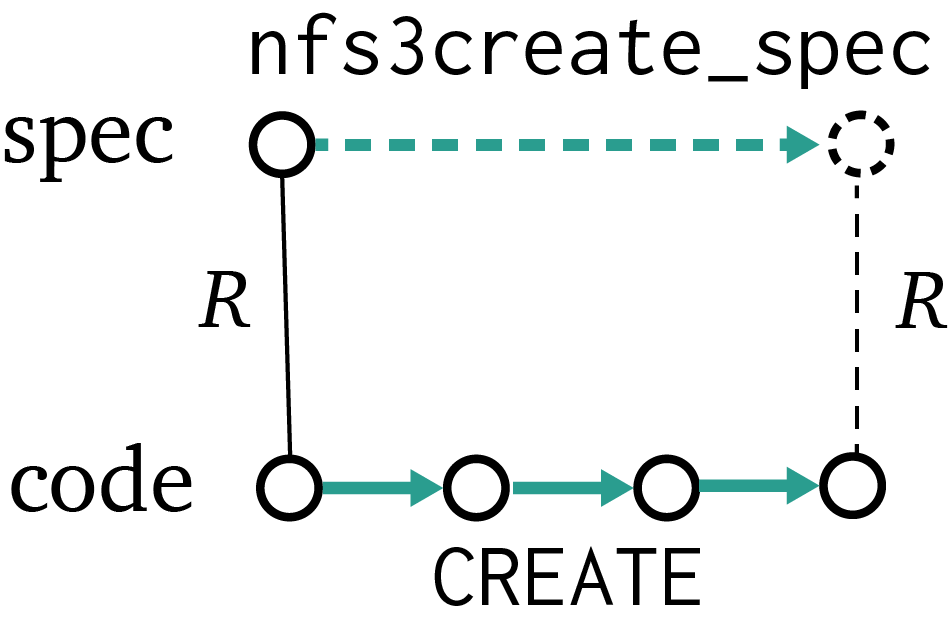
\includegraphics{fig/sequential-refinement.png}
  \end{subfigure}~~~~~\vrule~~~~%
\begin{subfigure}{0.3\textwidth}
  {\small
\begin{verbatim}

method CREATE(d_ino: uint64,
              name: Bytes)
 returns (r: Result<Ino>)
 requires R(txn_disk, fs)
 ensures R(txn_disk, fs)
 ensures r.Ok? ==>
 nfs3create_spec(d_ino, name,
   old(fs), fs, r.v)
\end{verbatim}
}
  %\caption{Dafny encoding}%
  %\label{fig:refinement:dafny}
\end{subfigure}
\vspace{0.5\baselineskip}
  \caption[Illustration of sequential refinement and its Dafny encoding]%
  {Illustration of $\seqrefinement(\infs)$ (left) and its encoding
in Dafny $\seqrefinementdfy(\infs)$ (right), for one particular operation.
In the diagram, the solid parts are assumed, and the
dashed parts must be shown to exist. The complete Dafny spec is more precise about
errors.}
  \label{fig:refinement}
\end{figure}

% hack to get theorem to have same number as original (only works because that's
% the first theorem, and there are no subsequent theorems)
\setcounter{theorem}{0}

We can now take simulation transfer and the Dafny proof and combine them to get
the overall DaisyNFS correctness theorem:
\begin{theorem}[DaisyNFS correctness, restated]
  DaisyNFS atomically implements the NFS protocol, formally stated as the
  refinement $\linkedcode \refines \snfs$. Note that
  $\sdfy = \mathrm{link}(\snfs, \infs)$. The system must be initialized with the
  \cc{Init} constructor on an empty disk, and then after every reboot
  re-initialized with the \cc{Recover} constructor.
  \label{thm:daisy-correctness-restatement}
\end{theorem}

This theorem re-states the specification developed in
\cref{sec:daisy:refinement-spec}. Its proof is a simple on-paper argument that
connects \cref{thm:gotxn-transfer} (which \emph{assumes} a sequential
refinement) to \cref{thm:dafny} (which \emph{proves} this sequential refinement).
\Cref{fig:refinement-execs} illustrates
the intuition for this theorem in terms of an example execution of $\snfs$: the transaction system proof guarantees an
atomic execution while the sequential refinement guarantees the transactions
themselves are correct.

\begin{figure}
  \centering
  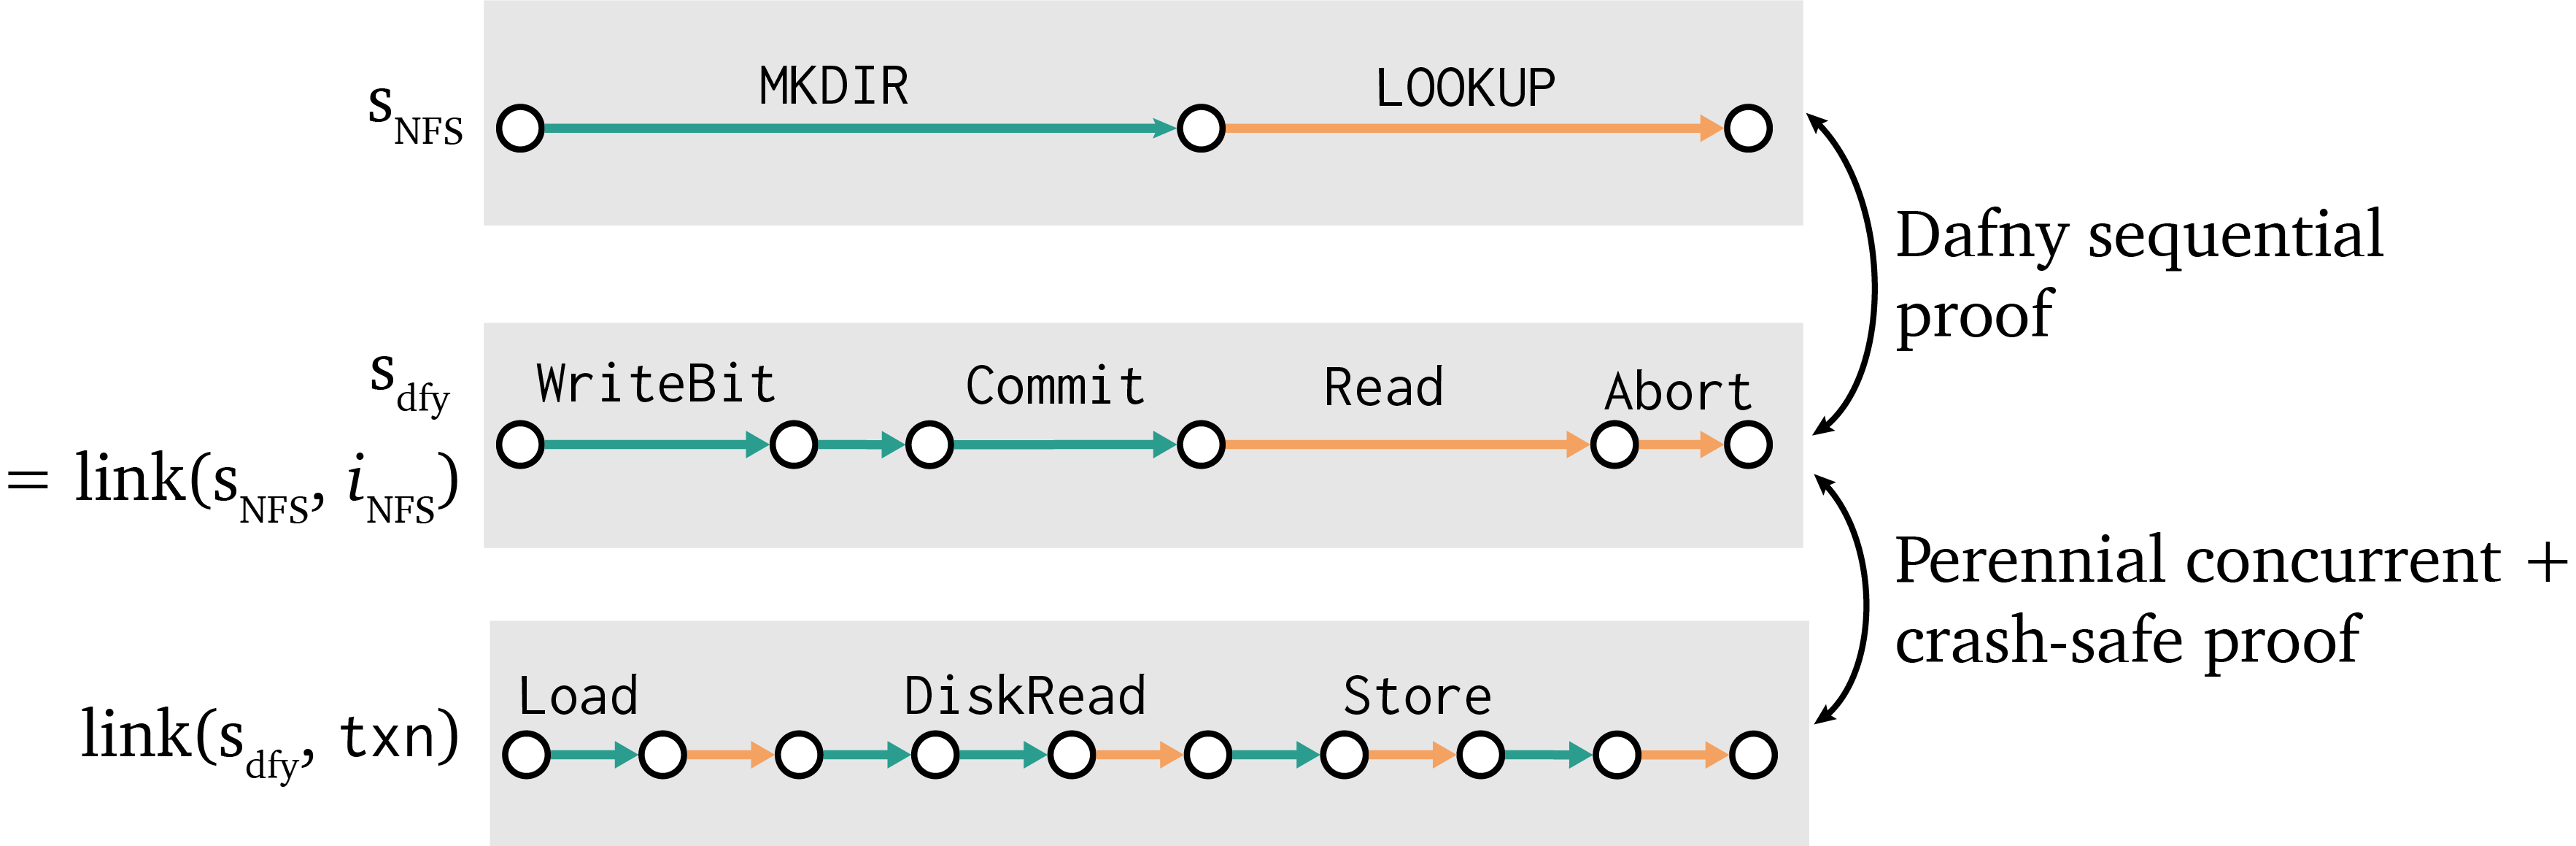
\includegraphics{fig/refinement-execs.png}
  \caption[Overall DaisyNFS proof strategy]{Illustration of the DaisyNFS proof
    strategy in terms of one
    possible execution of DaisyNFS, receiving parallel \cc{MKDIR} and \cc{LOOKUP}
    operations, at its three abstraction levels. Operations in each row are
    color-coded green or orange according to which operation they correspond to
    (the top-level \cc{MKDIR} or \cc{LOOKUP} respectively). The refinement proof first
    shows that for every code execution (bottom row), there exists an atomic
    execution at the Txn layer (middle row), as proven in
    \cref{thm:gotxn-transaction-refinement}. This justifies sequential reasoning to
    show the transactions on top follow the NFS specification (top row), as
    proven in \cref{thm:dafny}. Putting the two together,
    \cref{thm:daisy-correctness-restatement} shows the entire DaisyNFS server atomically
    implements the NFS specification.}
  \label{fig:refinement-execs}
\end{figure}

There are two assumptions needed for the theorems to compose. First,
$\seqrefinement_{\mathrm{dfy}}(i_{NFS})$ should imply $\seqrefinement(i_{NFS})$,
to bridge the assumption and theorem being proven in Dafny. That is, the
encoding of the refinement conditions in Dafny must be correct, but also the
semantics of the transaction system operations modeled in Dafny must match the
Coq proof. Second, every Dafny transaction must be valid, meaning
$\safe(i_{NFS}(op))$. Safety has a static restriction that transactions
should not modify global state, which the Dafny code satisfies because the only
mutable state in the file-system Dafny class is the transaction system, so
file-system operations cannot make mutations other than through GoTxn. The
dynamic restrictions for safety are expressed with preconditions on the GoTxn
interface so that Dafny automatically enforces them.

% We have some
% confidence this holds due to a simple check over the Dafny code: the only
% mutable state in the Dafny class that implements the file system is the ghost
% variables and the transaction system, so it cannot make mutations other than
% through GoTxn (ghost variables cannot influence execution due to the design of
% Dafny).

\section{Verifying the Dafny implementation}%
\label{sec:daisy:design}

\Cref{sec:daisy:proof-dafny}
explains how DaisyNFS connects sequential verification in Dafny to concurrency
and crash safety in GoTxn. This instead section focuses on the sequential
verification and file-system design themselves.

% The proof is given by annotating the code with proof steps, which include
% updates to ghost state, assertions to assist the automated verification, and
% calls to lemmas.

DaisyNFS is implemented and verified in several layers of abstraction, depicted
in \cref{fig:dafny-layers}. Each layer is implemented as a class that wraps the
lower layer as a field, until finally the transaction system is an assumed interface in Dafny.
The \cc{daisy-nfsd} binary implements the NFS wire protocol in
unverified Go code and calls the top-level Dafny class and its verified
methods to handle each operation.

\begin{figure}
\small \centering
\begin{tabular}{ll}
  \toprule
  \textbf{Layer} & \textbf{Functionality} \\
  \midrule
  daisy-nfsd & NFS wire protocol. \\
  dir & Directories and top-level NFS API. \\
  typed & Inode allocation. \\
  byte & Implement byte-level operations using blocks. \\
  block & Gather blocks for each file into a single sequence. \\
  indirect & Indirect blocks organized in a tree. \\
  inode & In-memory, high-level inodes; block allocation. \\
  txn & Assumed interface to external transaction system. \\
  \bottomrule
\end{tabular}
\caption{Layers in the Dafny implementation and proof of the file-system
operations.}
\label{fig:dafny-layers}
\end{figure}

The layers of the file system
can be organized into groups that implement three difficult pieces of
functionality: organizing data blocks into metadata and data (the
indirect and block layers), translating byte-level operations into
block operations (the byte and typed layers), and implementing
directories as special files that the file system itself reads and
writes (the dir layer). The modularity was essential to complete the proof in
manageable chunks (to avoid overwhelming the developer and prover), and it would
have been natural even without verification.

\subsection{Implementing the file system using transactions}

The design of DaisyNFS is broadly similar to the file system in xv6~\cite{xv6},
as well as Yggdrasil~\cite{sigurbjarnarson:yggdrasil}, a verified sequential
file system. We also adopt the recursive strategy for implementing and
verifying indirect blocks from DFSCQ~\cite{akonradi-meng}; recursion simplifies
the implementation of triply-indirect blocks, which are needed to reach a
reasonable maximum file size of 512GB.\@ Unlike most file systems, DaisyNFS is designed
to fit every operation into a transaction in order to support our goal of
sequential reasoning. This is a non-standard design and we encountered some
unique challenges in doing so. In this section we highlight difficulties in
fitting two features into transactions: rename and freeing space from deleted
files.

\subsubsection{Rename}
\label{sec:dafny:rename}

The NFS RENAME operation is similar to the \cc{rename} system call: it moves a
source file or directory to a destination location. What makes it tricky is that
it involves more than one inode and hence introduces the possibility for
deadlock.
% , which we would like to avoid even if the theorems do not forbid it.
We
use the standard strategy of enforcing a global ordering where inodes are always
locked in numerical order (smaller inode numbers first); this avoids a deadlock
where a cycle of threads is waiting on each other.

In a rename operation, the source and destination are each specified by a
combination of the parent directory inode and name within that directory. Rename
has an additional functionality of overwriting the destination if the source and
destination are files, or if both are directories and the destination is empty.
It is this latter check that makes deadlock avoidance difficult: it is necessary
to lock the source and destination directories first to lookup the source and
destination names, but those might be files that are earlier in the inode lock
order. We address this in the code by returning an error from the Dafny
transaction before the lock order would be violated. The error comes with the
set of inodes that should have been acquired.  The rename is then re-run with
this set of inodes as a lock hint which are all acquired in the correct
order at the beginning of the operation. The inodes to lock are only a hint and must be compared
against the current source and destination in case those inodes have changed in
the mean time. The rename operation runs in a loop until the lock hint succeeds;
the loop is potentially unbounded, but each iteration can only fail due to
concurrent renames that involve the same inodes.

At this point it is worth discussing the performance considerations that lead to
handling lock ordering in the file
system, rather than generically in GoTxn. The transaction system could
avoid deadlocks by either enforcing a global order over addresses or by
timing-out operations. Enforcing a global order is inefficient for the file
system; data blocks will never cause deadlock because the file system only
accesses a block after locking the (unique) inode that owns it. Timing-out
operations would lead to slow and spurious transaction failures that could more
rapidly be avoided in the higher-level code, hence we do not attempt to detect
deadlock dynamically.


\subsubsection{Freeing space}
\label{sec:dafny:freeing}

Freeing space becomes surprisingly tricky with large files. The problem is that
a large-enough file may reference too many blocks to be
freed in a single transaction. Transactions are bounded by the size of the
on-disk log (which can hold 511 blocks), whereas freeing a file requires
writing 0s to the block allocator for all of its formerly used blocks to mark them as free.
DaisyNFS handles this issue by splitting file removal and space reclamation
into separate transactions. The latter is implemented with an operation
\cc{ZeroFreeSpace(ino)} which frees and zeros the unused space in an inode that
we prove has no effect on the logical file-system state. Because this operation is a
logical no-op, it is safe to call it at any time.

The implementation is careful to call \cc{ZeroFreeSpace} after any operation
that leaves unused blocks, in particular \cc{REMOVE}, which deletes a file, and
\cc{SETATTR}, which can shrink a file by reducing its size. Since
\cc{ZeroFreeSpace} doesn't affect the user-visible data, it can return early to
avoid overflowing a transaction. The unverified code that manages freeing space
runs the operation in a loop until it covers all of the unused space in an
inode.

There is one case where freeing blocks is important for correctness and not just
to reclaim space. Growing a file is supposed to logically fill the new space
with zeros. If the file had old data in that space, it might not be zero but
instead contain previously written and deleted data, which both violates the specification and
is a potential security risk. The way we handle this with background freeing is
with validation: when the \cc{SETATTR} operation grows a file, it checks if the
free space is already zero first, and if not fails with a special error code. The
unverified code uses this error as a signal to immediately call
\cc{ZeroFreeSpace} and try the operation again. The same support also handles
holes created by writing past the end of a file, which are similarly supposed to
be zero.

The freeing implementation is an interesting example of using validation in
verification. The specification for much of the freeing code is loose, allowing
any data to be written to the free space. Only the code that checks if the
zeroing is done needs to be verified against a strong specification. The rest of
the code does still needs to be correct for this check to succeed, but we
aren't required to prove it.

\subsection{Verifying the indirect block implementation}%
\label{sec:dafny:indirect}

DaisyNFS supports large files using indirect blocks. A file's inode has a fixed
number of addresses for block addresses, some of which are used as indirect
blocks that hold another layer of addresses rather than direct blocks that have
file data. A single level of indirection is insufficient for a practical file
system, so DaisyNFS implements support for arbitrarily indirect blocks, and in
practice the file system uses up to triply-indirect blocks to support files up
to 512GB.\@

The indirect and block layers together implement an abstraction of a file as a
sequence of blocks, hiding the fact that some of the blocks are used as
metadata. These sequences are always of the maximum size, and only the next
layer reasons about file sizes. To efficiently represent files of the maximum
size, the code uses a convention that a zero block address is treated implicitly
as encoding a zero block, including for indirect blocks, an idea borrowed from
DFSCQ~\cite{akonradi-meng}. Indirect blocks are implemented recursively, where a
$k$-indirect block is always treated as containing 512 pointers to
$(k-1)$-indirect blocks, and a 0-indirect block contains file data. Zeros are
also treated recursively so that a single zero in an inode for the root of a
triply-indirect block efficiently stores a whole tree corresponding to many
gigabytes of zeros.

An inode has space for twelve 64-bit block addresses, after accounting for space
used by its attributes and type information. In principle all of these addresses
could be uniformly used as triply-indirect blocks. However, this would create a
lot of indirection for small files and lower performance for the common case.
Thus instead of organizing them in this way, the code uses a whole range, with
mostly direct blocks and a handful of indirect blocks. To keep the code general,
the indirection level of each of the twelve blocks is given in a global
indirect-block configuration, and most of the code is generic over the configuration. We currently
configure DaisyNFS with 8 direct blocks, two 1-indirect blocks, a 2-indirect
block, and a 3-indirect block. Just the direct and indirect blocks can address 4
MB fairly efficiently, but the triply-indirect block allows files to be large.

Indirect blocks pose a challenge for verification due to the classic problem of
\emph{aliasing}. The proof must show that modifying a data block or indirect
block has no effect on other files. In the DFSCQ proof, the invariant
captures the non-aliasing between files using separation logic, which makes
disjointness easy to express. In Dafny we have no such logical
technique, so we instead use a standard SMT-friendly trick for the invariant: in
addition to the physical mapping that tracks how to dereference a block address,
the indirect layer proof tracks a ghost \emph{reverse} mapping that tracks where
each in-use block number is stored. The invariant states that the forward and reverse
mappings are inverses of each other, which implies that modifying an address
only affects its owner and nothing else.

To encode the reverse mapping, the code uses a ``position'' datatype \cc{Pos} to
represent the location of a block within an inode. With indirect blocks, the
metadata blocks themselves also need to be considered locations, since the
invariant must also rule out metadata aliasing with data or other metadata. A
\cc{Pos} encodes an inode, an indirection level, and an offset for the blocks at
that indirection level to uniquely identify where a block is used. If we imagine
that an inode's block pointers are organized in a tree, the roots are stored
directly in the inode while the leaves are direct blocks. An indirection level
which is higher than the leaf level describes a metadata block.

The indirect block proof is split into the indirect and blocks layers. In the
indirect layer, the abstract state maps a \cc{Pos} to a block, and separately
tracks the size and attributes of each inode. The invariant also expresses that
the block allocator's used blocks have an associated \cc{Pos} and that the free
ones do not. The interface for the indirect layer exposes reads and writes for
positions, regardless of whether they are metadata or data blocks. The block
layer above instead exposes a map from inode number to a flat sequence of blocks by
mapping each leaf position to its linear index within the inode. Separating
these two made it easier to work on the indirect layer while exposing a much
more natural abstraction of a file as a sequence of blocks for the rest of the
file-system implementation.


% \subsection{Random notes on development process}
%
% \begin{itemize}
%   \item Used inefficient functional Dafny code at first, then slowly migrated to
%         in-memory data structures and improved performance.
%   \item Hard to debug and fix timeouts. Profiling verification performance is
%         hard.
%   \item Profiling Go code is great as usual. The generated code looks strange,
%         but I think after code generation it's pretty ordinary (the weird things
%         are mostly bad variable names, lot of unused assignments, and anonymous
%         functions that are immediately called).
%   \item Used some unit tests, but very few and only at the top level. Mainly
%         debugged Go compilation issues and cases where errors were
%         unintentionally being returned.
%   \item Trusted code isn't easy, had bugs in it before testing it thoroughly.
%         Also violated preconditions in top-level specs, triggering memory-safety
%         bugs.
% \end{itemize}

